\documentclass[conference]{IEEEtran}
\IEEEoverridecommandlockouts

\usepackage{cite}
\usepackage{amsmath,amssymb,amsfonts}
\usepackage{graphicx}
\usepackage{textcomp}
\usepackage{xcolor}
\usepackage{booktabs}
\usepackage{array}
\usepackage{tikz}
\usetikzlibrary{shapes.geometric, arrows.meta, positioning}
\usepackage[hidelinks]{hyperref}

\graphicspath{{figures/}}

\begin{document}

\title{Explainable Multi-Class Anemia Classification from Complete\\
Blood Count Data: A Detailed Study of Tree-Ensemble Models,\\
Their Training, and Per-Prediction SHAP Interpretation}

\author{
\IEEEauthorblockN{Aditya Dhull}
\IEEEauthorblockA{\textit{Independent Study in Applied Machine Learning} \\
\texttt{adityadhull@iisc.ac.in}}
}

\maketitle

\begin{abstract}
Anemia is among the most common hematologic conditions worldwide, and its many
subtypes---each with distinct causes and treatments---are reflected in the
inexpensive, ubiquitous Complete Blood Count (CBC). We present a detailed,
reproducible, and explainable framework that classifies patients into nine
diagnostic categories from $14$ CBC parameters ($n{=}1{,}232$ after removing
duplicate records). We study five tree-ensemble models in depth---Random Forest,
XGBoost, a soft-voting hybrid of the two, LightGBM, and a stacking ensemble---
giving the learning principle, optimisation objective, and exact training
procedure of each, together with a leakage-safe preprocessing and
cross-validation methodology. The soft-voting hybrid attains a hold-out accuracy of
$0.984$ and macro-F1 of $0.947$, while a stacking ensemble attains the best
cross-validated macro-F1 ($0.966$). A paired
$t$-test finds the hybrid's improvement over the Random-Forest baseline is
\emph{not} statistically significant ($p{=}0.82$); we further show, via a
seed-stability analysis, that a five-fold paired $t$-test p-value ranges from
$0.03$ to $0.99$ on these data, so only the qualitative verdict is robust. Exact
TreeSHAP yields global attributions that recover the mean-corpuscular-volume
morphological framework (HGB, MCV, MCH, MCHC, PLT lead) and per-prediction
explanations that match hematologic reasoning; in one case SHAP exposes a
physiologically impossible record, demonstrating interpretability as a
data-quality tool.
\end{abstract}

\begin{IEEEkeywords}
Anemia, Complete Blood Count, Random Forest, XGBoost, LightGBM, stacking, soft
voting, SHAP, explainable AI, statistical significance.
\end{IEEEkeywords}

\section{Introduction}
A Complete Blood Count quantifies the cellular components of blood---red cells,
white cells, and platelets---and is one of the most frequently ordered laboratory
tests. Because the morphology of red cells encodes the \emph{cause} of an anemia,
the CBC supports not merely the detection of anemia but the discrimination of its
subtypes, which carry different clinical management (iron supplementation, vitamin
replacement, hematology referral). Automated multi-class classification of these
subtypes can therefore assist triage and decision support.

This paper presents and details a hybrid Random-Forest\,$+$\,XGBoost soft-voting
framework for nine-class anemia classification, and goes beyond a results table in
two respects. First, we give a thorough account of \emph{every} model used and
exactly how it is trained---the bagging and boosting principles, the regularised
boosting objective, the voting and stacking combination rules, and the precise
hyperparameters and imbalance handling. Second, we provide per-prediction SHAP
explanations and a rigorous treatment of statistical significance, including a
demonstration that a small-sample p-value is itself unstable. Our contributions are
a detailed comparative treatment of five tree ensembles and their training; a
careful evaluation including an honest non-significant model comparison; and exact
global and instance-level SHAP explanations, one of which reveals a data-quality
error.

\section{Clinical Background}
\subsection{Blood and the CBC}
Blood comprises red blood cells (erythrocytes, carrying hemoglobin), white blood
cells (leukocytes, immune defence), and platelets (thrombocytes, clotting). The
$14$ CBC features used here are the white-cell count (WBC), lymphocyte and
neutrophil percentages and absolute counts (LYMp, NEUTp, LYMn, NEUTn), red-cell
count (RBC), hemoglobin (HGB), hematocrit (HCT), the red-cell indices mean
corpuscular volume (MCV), mean corpuscular hemoglobin (MCH) and its concentration
(MCHC), platelet count (PLT), platelet distribution width (PDW), and plateletcrit
(PCT).

\subsection{The Morphological Framework}
Anemia is a deficiency of hemoglobin. Its \emph{cause} is classically inferred from
red-cell size and colour. \textbf{MCV} partitions anemias into microcytic
(small, MCV${<}80$\,fL), normocytic (normal, $80$--$100$\,fL) and macrocytic
(large, ${>}100$\,fL); \textbf{MCH}/\textbf{MCHC} add the hypochromic-versus-
normochromic (pale-versus-normal) axis. This two-dimensional logic is precisely why
a model trained on the CBC concentrates its attention on MCV, MCH, MCHC and HGB---a
prediction we verify with SHAP.

\subsection{The Nine Target Classes}
The dataset's classes are \textit{Healthy}; \textit{Iron deficiency anemia}
(microcytic, hypochromic; low MCV/MCH/MCHC); \textit{Other microcytic anemia}
(e.g.\ thalassemia or chronic disease, microcytic with a different pattern);
\textit{Macrocytic anemia} (high MCV; B12/folate deficiency); \textit{Normocytic
normochromic anemia} (normal indices, low HGB; e.g.\ chronic disease, renal,
acute loss); \textit{Normocytic hypochromic anemia}; \textit{Thrombocytopenia}
(low PLT); \textit{Leukemia} (abnormal WBC); and \textit{Leukemia with
thrombocytopenia}. The platelet and white-cell features discriminate the last
three from the red-cell anemias.

\section{Dataset and Preprocessing}
The dataset (\texttt{diagnosed\_cbc\_data\_v4}) contains $14$ numeric CBC features
and a nine-class diagnosis. We remove exact duplicate records to avoid
performance inflation, leaving $1{,}232$ patients. The
class distribution (Fig.~\ref{fig:dist}) is moderately imbalanced: the three
largest classes (Healthy, the two normocytic anemias) account for the majority,
while Macrocytic anemia and Leukemia-with-thrombocytopenia are rare ($\leq1.3\%$).
All features are numeric, so preprocessing reduces to median imputation (with a
missing-indicator for completeness, though this dataset has no missing values) and
the diagnosis is integer-encoded. As tree ensembles are invariant to monotone
scaling, no standardisation is applied. The transform is wrapped in a
\texttt{ColumnTransformer} fit only on training data (Section~\ref{sec:leak}).

\begin{figure}[t]
\centering

\includegraphics[width=0.95\columnwidth]{anemia_class_dist.png}
\caption{Class distribution of the nine anemia categories after de-duplication.}
\label{fig:dist}
\end{figure}

\section{Models}
All five models are tree-based: trees handle the CBC's numeric thresholds
natively, need no scaling, capture the non-linear index logic of hematologic
diagnosis, and admit \emph{exact} SHAP explanations. We describe each in turn.

\subsection{Foundation: the Decision Tree}
A decision tree recursively splits feature space on the feature/threshold that
most reduces node impurity, measured by the Gini index $G=1-\sum_c p_c^2$ or
entropy. A leaf predicts its training samples' class distribution. A single deep
tree is low-bias but high-variance (it overfits); the ensembles below reduce
variance and bias in complementary ways.

\subsection{Random Forest (Bagging)}
A Random Forest averages $T$ decorrelated trees,
\begin{equation}
f_{\mathrm{RF}}(x)=\frac{1}{T}\sum_{t=1}^{T}h_t(x),
\end{equation}
each grown on a bootstrap resample and using a random feature subset
($\approx\sqrt{d}$) at every split. With per-tree variance $\sigma^2$ and pairwise
correlation $\rho$, the average's variance is
$\rho\sigma^2+\tfrac{1-\rho}{T}\sigma^2$, so decorrelation (small $\rho$) and many
trees ($T$) reduce variance without raising bias---the \emph{bagging} principle.
Multi-class trees output class distributions that the forest averages into
probabilities. We use $T{=}300$ trees with \texttt{balanced\_subsample} class
weights.

\subsection{XGBoost (Gradient Boosting)}
Boosting reduces bias by adding trees sequentially, each correcting its
predecessors: $\hat{y}_i^{(t)}=\hat{y}_i^{(t-1)}+f_t(x_i)$. XGBoost minimises the
regularised objective
\begin{equation}
\mathcal{L}^{(t)}=\sum_{i=1}^{N}\ell\!\left(y_i,\hat{y}_i^{(t-1)}+f_t(x_i)\right)
+\Omega(f_t),\;\;\Omega(f)=\gamma T+\tfrac{\lambda}{2}\sum_j w_j^2 .
\end{equation}
A second-order Taylor expansion with gradients $g_i$ and Hessians $h_i$ yields the
optimal leaf weight and structure score
\begin{equation}
w_j^\star=-\frac{G_j}{H_j+\lambda},\qquad
\tilde{\mathcal{L}}=-\frac{1}{2}\sum_j\frac{G_j^2}{H_j+\lambda}+\gamma T,
\end{equation}
with $G_j=\sum_{i\in I_j}g_i,\;H_j=\sum_{i\in I_j}h_i$, and a split is kept only if
its gain
\begin{equation}
\tfrac{1}{2}\!\left[\frac{G_L^2}{H_L+\lambda}+\frac{G_R^2}{H_R+\lambda}
-\frac{(G_L+G_R)^2}{H_L+H_R+\lambda}\right]-\gamma
\end{equation}
is positive---this is how $\lambda,\gamma$ regularise at the split level. We use
the multi-class softmax objective, $400$ trees of depth $6$, learning-rate
$0.1$, row/column subsampling $0.9$, $\lambda{=}1$, the histogram split-finder, and
balanced per-sample weights (Section~\ref{sec:imb}).

\subsection{The Hybrid: Soft Voting}
The hybrid averages the forest's and the booster's posterior probabilities,
\begin{equation}
\hat{y}=\arg\max_{c}\frac{1}{M}\sum_{m=1}^{M}P_m(c\mid x),\qquad M=2,
\end{equation}
combining variance reduction (forest) and bias reduction (booster). Soft voting
weights each model by its confidence; partly uncorrelated errors cancel. Both
learners share one preprocessing transform, ensuring identical inputs.

\subsection{LightGBM}
LightGBM is a gradient booster using \emph{leaf-wise} (best-first) growth,
histogram binning, gradient-based one-side sampling, and exclusive-feature
bundling for speed and accuracy. We use $400$ trees, $63$ leaves, learning-rate
$0.05$, and \texttt{balanced} class weights.

\subsection{Stacking}
Stacking \emph{learns} the combination rather than fixing equal weights. Level-0
learners (Random Forest, XGBoost, LightGBM) produce \emph{out-of-fold} probability
predictions (via internal $5$-fold CV, hence leakage-free) that feed a level-1
multinomial logistic-regression meta-learner with balanced weights. The
meta-learner can weight base models differently per class, an adaptivity beyond
fixed voting, at the cost of more computation.

\section{Training Methodology}
\subsection{Leakage-Safe Pipeline}
\label{sec:leak}
Each model is a \texttt{Pipeline} of preprocessing followed by a classifier;
fitting learns imputation statistics and encodings from the training partition
only, and cross-validation re-fits the whole pipeline per fold, so no held-out
statistic leaks into training (Fig.~\ref{fig:arch}).

\subsection{Stratified Splitting and Cross-Validation}
We use a stratified $80/20$ hold-out and stratified five-fold cross-validation on
the training partition; stratification preserves class proportions, essential when
the rarest class is ${<}1\%$ of data. We report mean$\pm$std across folds with
$\sigma=\sqrt{\tfrac14\sum_{j=1}^{5}(S_j-\mu)^2}$ and retain the individual fold
scores for the paired significance test.

\subsection{Class-Imbalance Handling}
\label{sec:imb}
Random Forest, LightGBM and the meta-learner use balanced class weights
$w_c=N/(K\,n_c)$; XGBoost receives the same correction as per-sample weights. With
macro-averaged metrics, rare anemia subtypes influence both training and scoring.

\subsection{Hyperparameters and Reproducibility}
Table~\ref{tab:hp} lists each model's configuration. All models share a fixed seed
($42$); the download, preprocessing, training, evaluation and figures run from one
scripted pipeline for end-to-end reproducibility.

\begin{table}[t]
\caption{Model hyperparameters.}
\label{tab:hp}
\centering
\footnotesize
\renewcommand{\arraystretch}{1.2}
\begin{tabular}{p{1.7cm}p{6cm}}
\toprule
\textbf{Model} & \textbf{Key settings} \\
\midrule
Random Forest & $300$ trees, unlimited depth, $\sqrt{d}$ features/split,
\texttt{balanced\_subsample} weights \\
XGBoost & $400$ trees, depth $6$, lr $0.1$, subsample $0.9$, colsample $0.9$,
$\lambda{=}1$, \texttt{multi:softprob}, hist, balanced sample weights \\
LightGBM & $400$ trees, $63$ leaves, lr $0.05$, subsample $0.9$, colsample $0.9$,
\texttt{balanced} weights \\
Hybrid & soft voting of the above RF and XGBoost ($M{=}2$, equal weights) \\
Stacking & base: RF, XGBoost, LightGBM; meta: multinomial logistic regression
($5$-fold out-of-fold features) \\
\bottomrule
\end{tabular}
\end{table}

\begin{figure}[t]
\centering
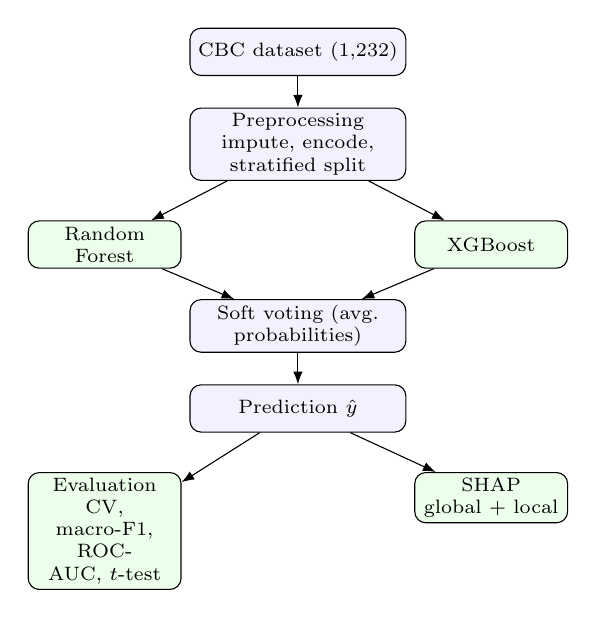
\begin{tikzpicture}[
  node distance=4mm and 6mm,
  box/.style={draw, rounded corners, align=center, font=\scriptsize,
              minimum height=6mm, inner sep=2pt, fill=blue!5, text width=26mm},
  base/.style={draw, rounded corners, align=center, font=\scriptsize,
              minimum height=6mm, inner sep=2pt, fill=green!8, text width=18mm},
  arr/.style={-{Latex[length=1.6mm]}}]
\node[box] (data) {CBC dataset (1{,}232)};
\node[box, below=of data] (prep) {Preprocessing\\impute, encode,\\stratified split};
\node[base, below left=5mm and 1mm of prep] (rf) {Random Forest};
\node[base, below right=5mm and 1mm of prep] (xgb) {XGBoost};
\node[box, below=15mm of prep] (vote) {Soft voting (avg.\ probabilities)};
\node[box, below=of vote] (pred) {Prediction $\hat{y}$};
\node[base, below left=5mm and 1mm of pred] (eval) {Evaluation\\CV, macro-F1,\\ROC-AUC, $t$-test};
\node[base, below right=5mm and 1mm of pred] (shap) {SHAP\\global $+$ local};
\draw[arr] (data) -- (prep);
\draw[arr] (prep) -- (rf);
\draw[arr] (prep) -- (xgb);
\draw[arr] (rf) -- (vote);
\draw[arr] (xgb) -- (vote);
\draw[arr] (vote) -- (pred);
\draw[arr] (pred) -- (eval);
\draw[arr] (pred) -- (shap);
\end{tikzpicture}
\caption{Leakage-safe training and evaluation pipeline. Preprocessing is fit
inside each cross-validation fold.}
\label{fig:arch}
\end{figure}

\section{Evaluation Protocol}
We report accuracy, balanced accuracy, macro-F1, and one-vs-rest ROC--AUC.
Macro-F1, the headline metric, averages per-class F1 equally so rare subtypes are
not masked by common ones:
\begin{equation}
\mathrm{Macro\text{-}F1}=\frac{1}{K}\sum_{i=1}^{K}
\frac{2\,\mathrm{Prec}_i\,\mathrm{Rec}_i}{\mathrm{Prec}_i+\mathrm{Rec}_i}.
\end{equation}
To test whether the hybrid beats the Random-Forest baseline we apply a paired
$t$-test to the fold-wise macro-F1 scores, $t=\bar{d}/(s_d/\sqrt{n})$, $n{=}5$, on
identical folds.

\section{Results}
\subsection{Cross-Validation and Model Comparison}
Table~\ref{tab:cv} and Fig.~\ref{fig:cmp} report five-fold cross-validation. The
hybrid attains macro-F1 $0.939$. All models exceed $0.98$ accuracy and $0.999$
ROC--AUC. Notably, the \emph{stacking} ensemble achieves the best cross-validated
macro-F1 ($0.966$)---the one configuration that clearly surpasses the soft-voting
hybrid, at the cost of higher training time.

\begin{table}[t]
\caption{Stratified five-fold cross-validation, mean\,$\pm$\,std.}
\label{tab:cv}
\centering
\renewcommand{\arraystretch}{1.2}
\begin{tabular}{lccc}
\toprule
\textbf{Model} & \textbf{Accuracy} & \textbf{Macro-F1} & \textbf{ROC-AUC} \\
\midrule
Random Forest     & $0.985\pm0.013$ & $0.934\pm0.055$ & $0.9996$ \\
XGBoost           & $0.988\pm0.004$ & $0.948\pm0.008$ & $0.9994$ \\
Hybrid (RF$+$XGB) & $0.987\pm0.007$ & $0.939\pm0.017$ & $0.9998$ \\
LightGBM          & $0.989\pm0.006$ & $0.947\pm0.053$ & $0.9997$ \\
Stacking          & $\mathbf{0.991\pm0.006}$ & $\mathbf{0.966\pm0.025}$ & $0.9998$ \\
\bottomrule
\end{tabular}
\end{table}

\begin{figure}[t]
\centering

\includegraphics[width=0.92\columnwidth]{anemia_model_cmp.png}
\caption{Mean cross-validated macro-F1 by model.}
\label{fig:cmp}
\end{figure}

\subsection{Statistical Significance and Its Instability}
The paired $t$-test of hybrid versus Random Forest gives $\bar{d}{=}{+}0.0053$,
$t{=}0.24$, $p{=}0.82$: \emph{not} significant. On roughly $1{,}200$ patients, the
hybrid's edge over a strong baseline lies within fold noise. To show that the exact
p-value is not itself a reliable quantity, we hold the data and models fixed and
vary only the fold-shuffling seed (Table~\ref{tab:pstab}); the p-value ranges from
$0.03$ to $0.99$, with nine of ten seeds non-significant and one crossing $0.05$ by
chance. Our $0.82$ is an unremarkable draw from this distribution: the robust
outcome is the \emph{verdict} (not significant), not any single number---a caution
against over-interpreting one statistic computed from five folds.

\begin{table}[t]
\caption{Hybrid-vs-RF paired $t$-test under different fold seeds (same data, same
models).}
\label{tab:pstab}
\centering
\renewcommand{\arraystretch}{1.15}
\begin{tabular}{cccc}
\toprule
\textbf{Seed} & \textbf{mean(Hyb$-$RF)} & \textbf{p-value} & \textbf{Verdict} \\
\midrule
13   & $+0.0002$ & 0.990 & not sig. \\
42   & $+0.0053$ & 0.824 & not sig. \\
0    & $+0.0067$ & 0.762 & not sig. \\
21   & $+0.0184$ & 0.425 & not sig. \\
7    & $+0.0204$ & 0.118 & not sig. \\
99   & $+0.0325$ & \textbf{0.029} & \textbf{significant} \\
\midrule
\multicolumn{4}{l}{\footnotesize Range over 10 seeds: $[0.029,\,0.990]$;
significant in $10\%$.} \\
\bottomrule
\end{tabular}
\end{table}

\subsection{Hold-Out Test Performance}
On the unseen $20\%$ test set the hybrid attains accuracy $0.984$, balanced
accuracy $0.939$, macro-F1 $0.947$, weighted-F1 $0.984$ and ROC--AUC $0.9997$.
Per-class results (Table~\ref{tab:pc}) show F1$\,\geq\,0.94$ for every
well-populated class and three classes at $1.00$; the only weak class is
Macrocytic anemia (F1 $0.667$ on just three test samples), a small-sample artifact
that illustrates the fragility of rare-class estimates. The confusion matrices
(Figs.~\ref{fig:cm},~\ref{fig:cmn}) are near-diagonal, and the ROC curves
(Fig.~\ref{fig:roc}) approach the ideal corner.

\begin{table}[t]
\caption{Per-class hold-out performance of the hybrid.}
\label{tab:pc}
\centering
\renewcommand{\arraystretch}{1.2}
\begin{tabular}{lcccc}
\toprule
\textbf{Class} & \textbf{Prec.} & \textbf{Rec.} & \textbf{F1} & \textbf{Sup.} \\
\midrule
Healthy                         & 0.985 & 1.000 & 0.992 & 65 \\
Normocytic hypochromic anemia   & 0.982 & 0.982 & 0.982 & 54 \\
Normocytic normochromic anemia  & 1.000 & 1.000 & 1.000 & 51 \\
Iron deficiency anemia          & 0.974 & 1.000 & 0.987 & 37 \\
Thrombocytopenia                & 1.000 & 1.000 & 1.000 & 15 \\
Other microcytic anemia         & 1.000 & 0.909 & 0.952 & 11 \\
Leukemia                        & 1.000 & 0.889 & 0.941 & 9 \\
Macrocytic anemia               & 0.667 & 0.667 & 0.667 & 3 \\
Leukemia with thrombocytopenia  & 1.000 & 1.000 & 1.000 & 2 \\
\midrule
macro avg                       & 0.956 & 0.939 & 0.947 & 247 \\
\bottomrule
\end{tabular}
\end{table}

\begin{figure}[t]
\centering
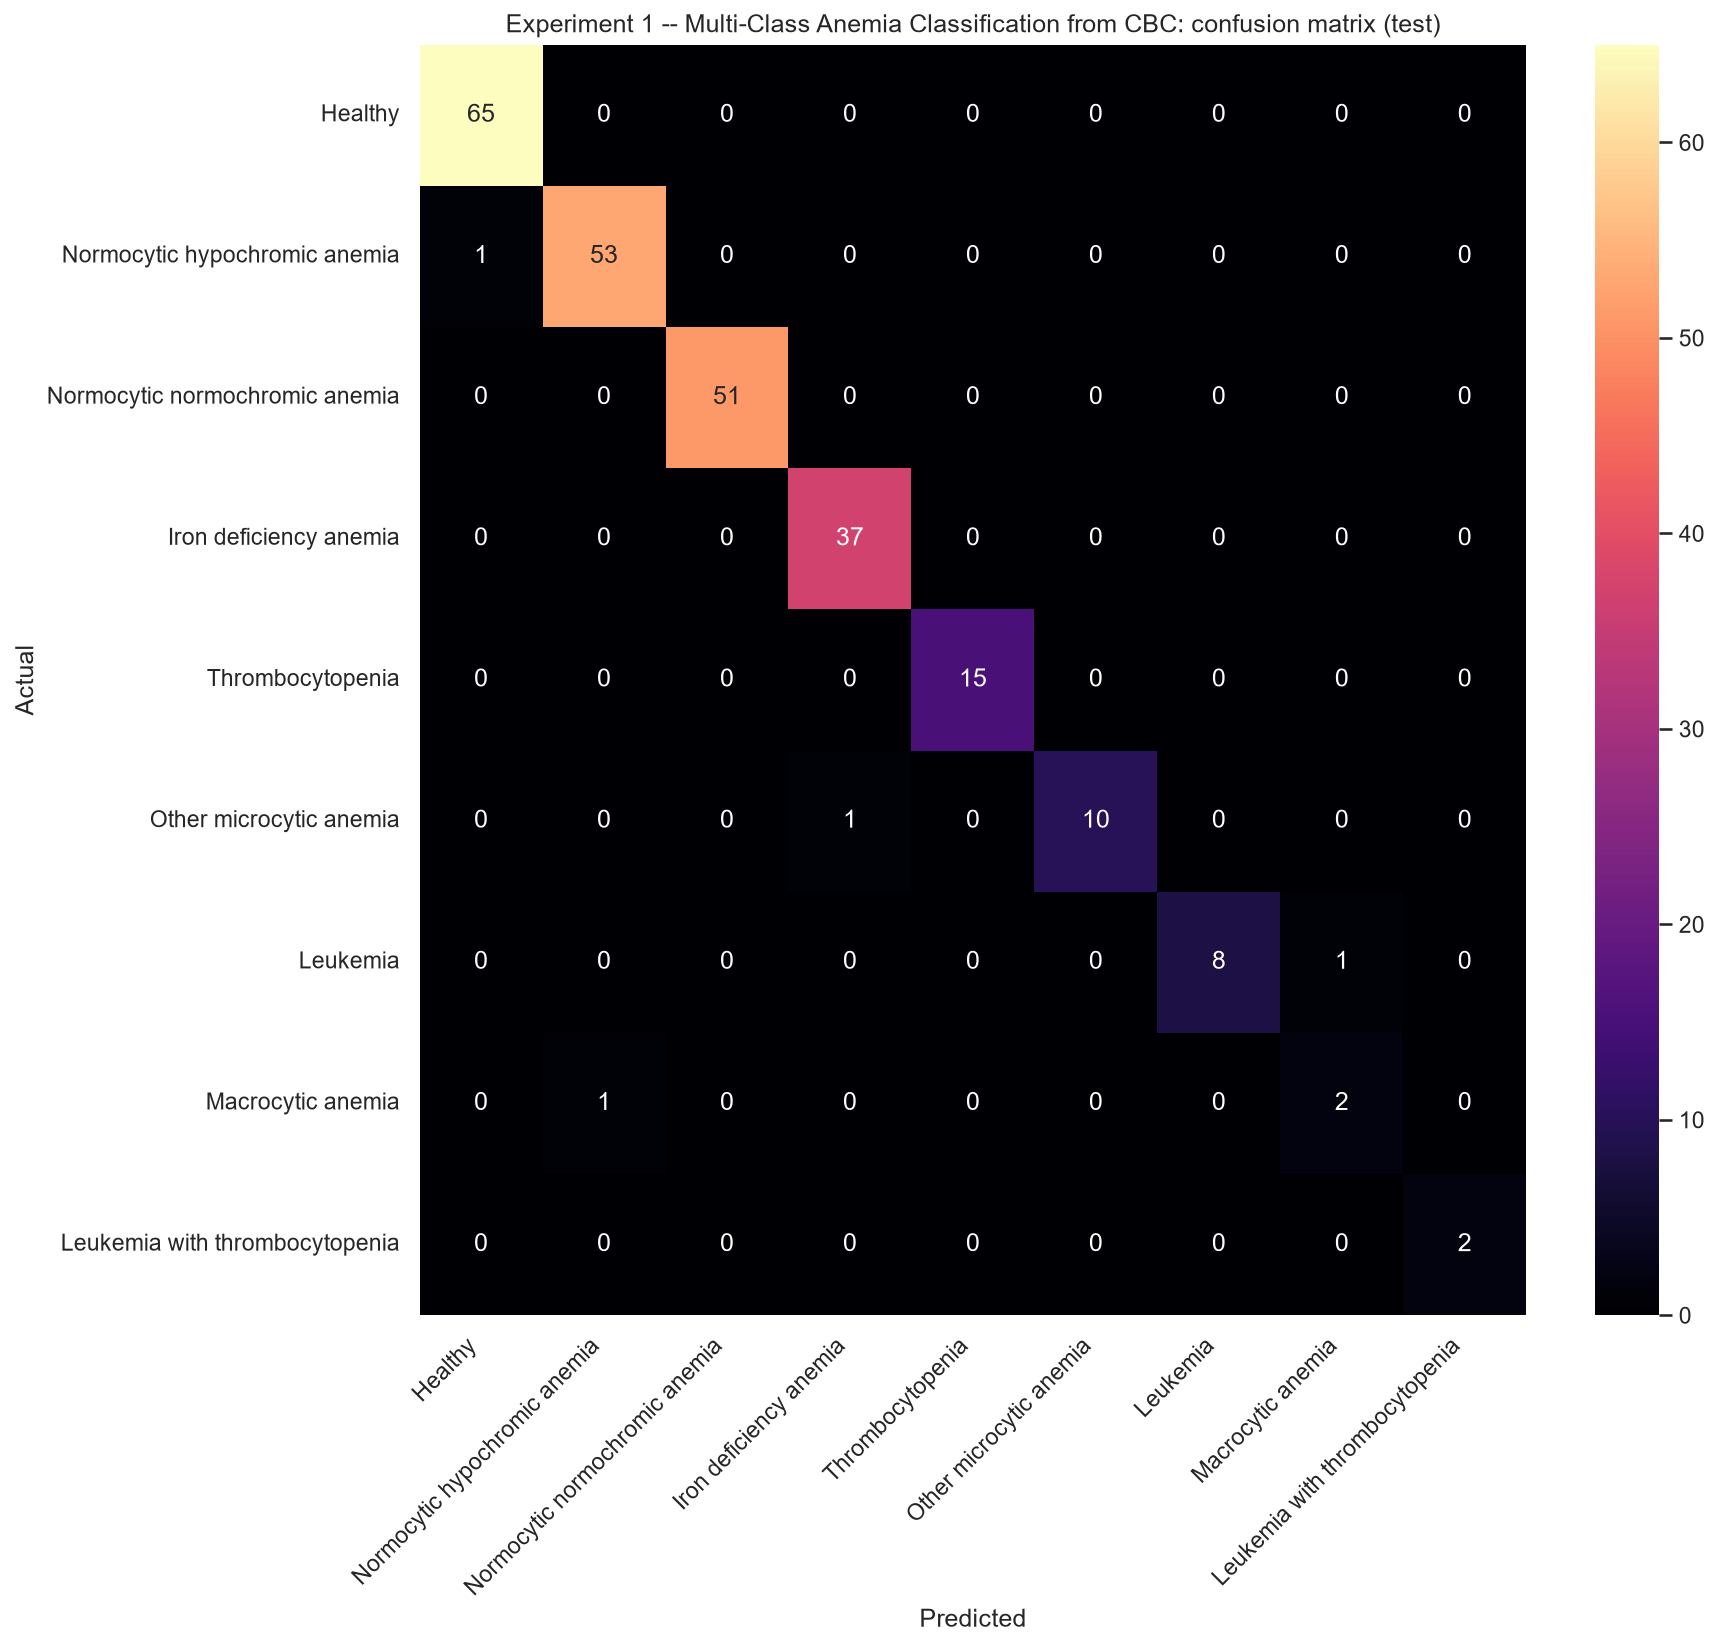
\includegraphics[width=0.95\columnwidth]{anemia_cm.png}
\caption{Confusion matrix of the hybrid on the anemia hold-out set (counts).}
\label{fig:cm}
\end{figure}

\begin{figure}[t]
\centering

\includegraphics[width=0.95\columnwidth]{anemia_cm_norm.png}
\caption{Row-normalised confusion matrix (per-class recall on the diagonal).}
\label{fig:cmn}
\end{figure}

\begin{figure}[t]
\centering

\includegraphics[width=0.92\columnwidth]{anemia_roc.png}
\caption{One-vs-rest ROC curves per class for the hybrid.}
\label{fig:roc}
\end{figure}

\section{Explainability}
\subsection{Global Attribution}
SHAP decomposes a prediction additively, $f(x)=\phi_0+\sum_j\phi_j$, with exact
TreeSHAP values. The global importances (Fig.~\ref{fig:shapbar}) are led by HGB,
MCV, WBC, MCHC, MCH and PLT---recovering the MCV-centred morphological framework
that underpins hematologic diagnosis. The SHAP \emph{interaction} summary
(Fig.~\ref{fig:bee}) splits each contribution into a main effect (the matrix
diagonal) and pairwise interactions (off-diagonal cells); the strongest cells
involve the red-cell indices MCV, MCH and MCHC, and the prominent
MCV$\times$MCH and MCV$\times$MCHC interactions encode the size-versus-colour logic
by which iron deficiency is distinguished. That the model's behaviour mirrors
hematologic teaching is strong evidence it learned signal, not artifact.

\begin{figure}[t]
\centering

\includegraphics[width=0.95\columnwidth]{anemia_shap_bar.png}
\caption{Global SHAP importance (mean $|\phi_j|$) of the XGBoost component.}
\label{fig:shapbar}
\end{figure}

\begin{figure*}[t]
\centering

\includegraphics[width=0.82\textwidth]{anemia_shap_interaction.png}
\caption{SHAP interaction-value summary for the iron-deficiency-anemia output. The
top seven features appear on both axes; each cell is a beeswarm of SHAP
\emph{interaction} values (x-axis), with colour encoding the feature value.
Diagonal cells are a feature's main effect; off-diagonal cells are pairwise
interactions.}
\label{fig:bee}
\end{figure*}

\subsection{Per-Prediction Explanations}
The additive decomposition narrates individual predictions. Two correct cases:
\begin{itemize}
\item \textbf{Iron deficiency anemia} (Fig.~\ref{fig:wf_iron}): a low MCV
($79.9$) and low MCH ($24.4$) drive the prediction---the microcytic, hypochromic
phenotype.
\item \textbf{Leukemia} (Fig.~\ref{fig:wf_leuk}): a markedly elevated white-cell
count (WBC${=}13.8$, ${+}3.65$) dominates, with the red-cell indices contributing
little---exactly the discriminating feature for this class.
\end{itemize}
Because the contributions sum to the model output, each explanation is complete and
auditable.

\subsection{Explaining Errors and Surfacing Data Quality}
SHAP on misclassified patients is diagnostically valuable. One patient labelled
\textit{Normocytic hypochromic} but predicted \textit{Healthy}
(Fig.~\ref{fig:wf_bug}) carries physiologically impossible values (HGB${=}41$,
RBC${=}13.1$, HCT${=}2$); the SHAP decomposition shows the absurd HGB drove the
error, turning a silent misclassification into a visible, diagnosable data-quality
problem. This exemplifies interpretability as a debugging tool, not merely a trust
signal, and motivates input range-checking before deployment.

\begin{figure}[t]
\centering
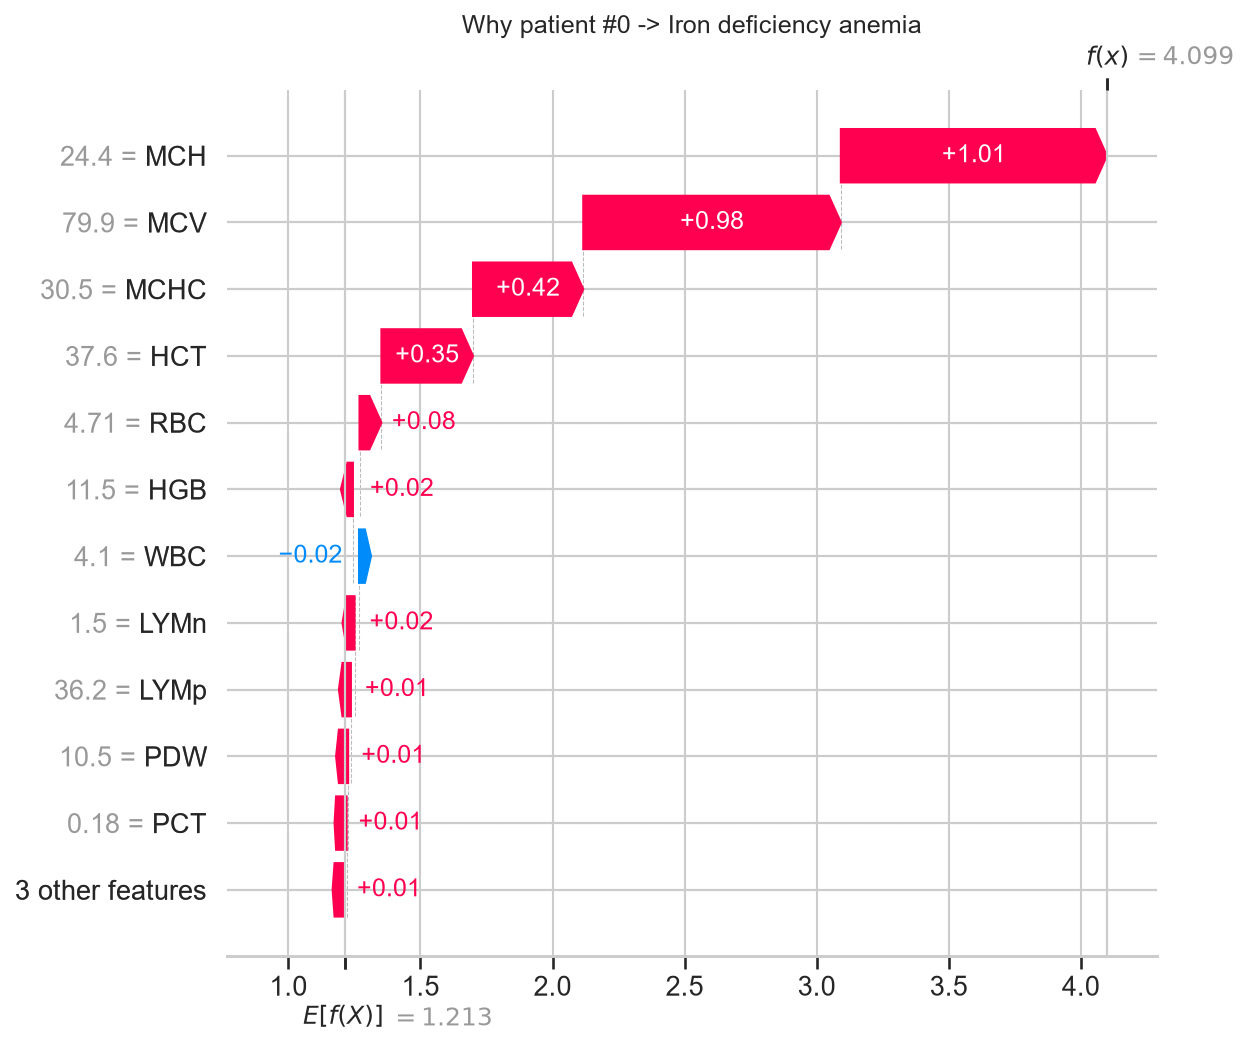
\includegraphics[width=0.97\columnwidth]{anemia_waterfall_iron.png}
\caption{Per-prediction SHAP waterfall: iron deficiency anemia. Low MCV and MCH
dominate.}
\label{fig:wf_iron}
\end{figure}

\begin{figure}[t]
\centering
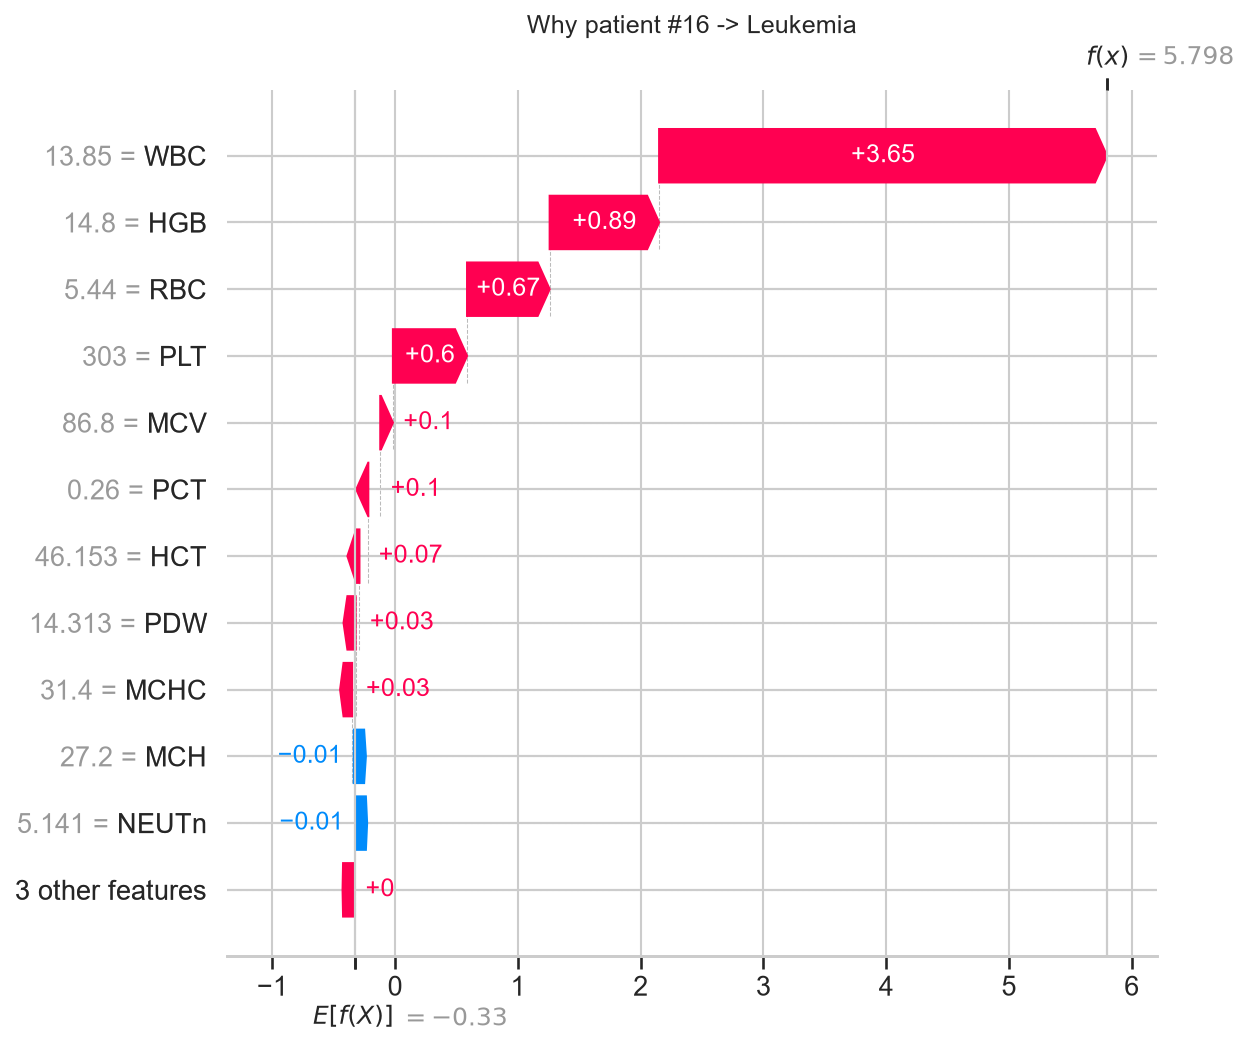
\includegraphics[width=0.97\columnwidth]{anemia_waterfall_leukemia.png}
\caption{Per-prediction SHAP waterfall: leukemia. The elevated WBC dominates.}
\label{fig:wf_leuk}
\end{figure}

\begin{figure}[t]
\centering
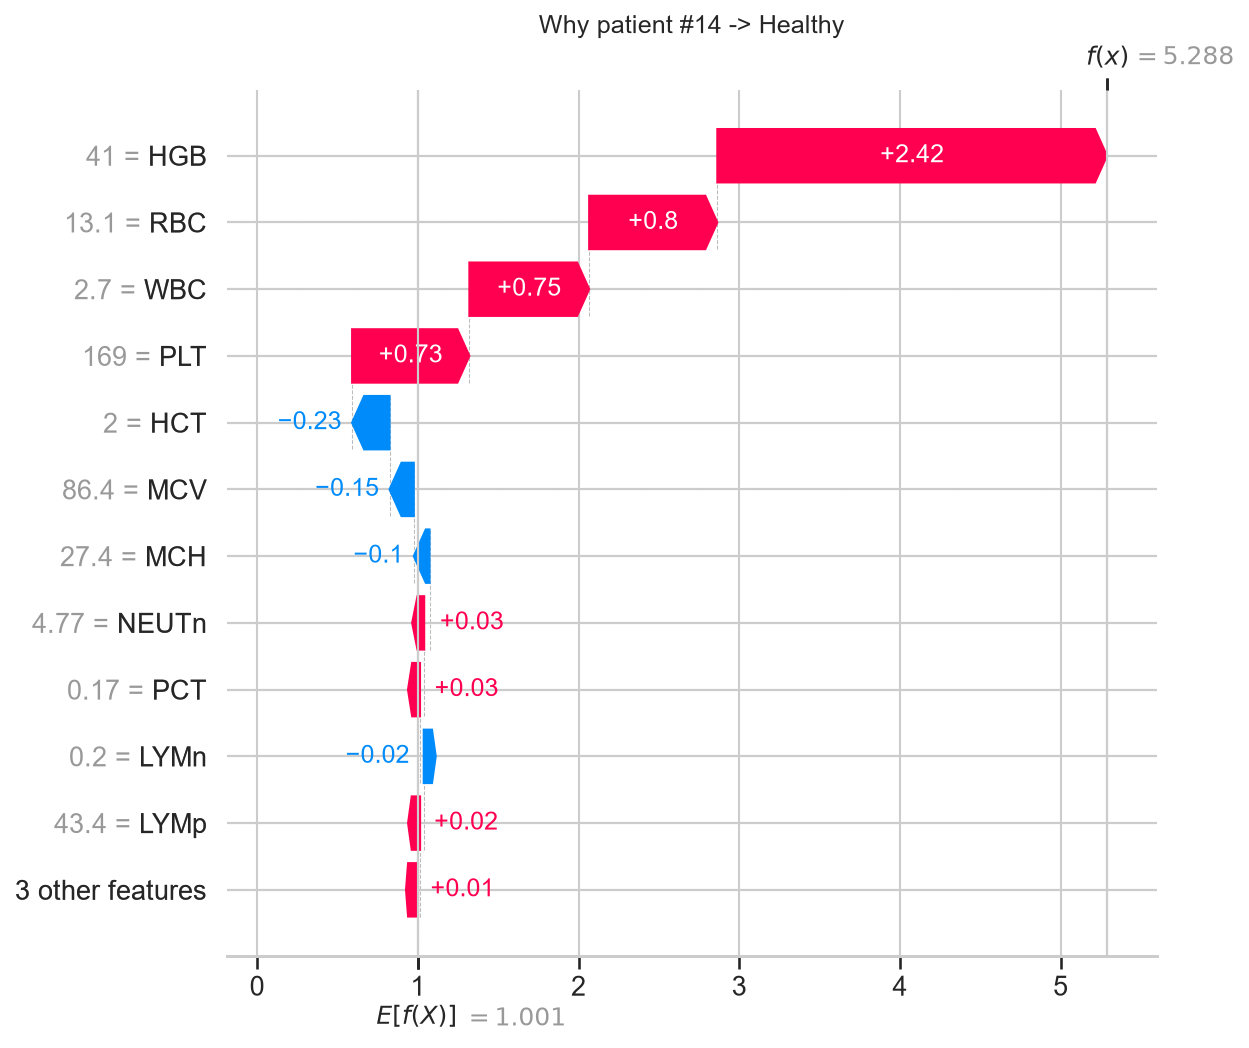
\includegraphics[width=0.97\columnwidth]{anemia_waterfall_dataquality.png}
\caption{A misclassified patient with impossible values (HGB${=}41$): SHAP exposes
the corrupt feature that misled the model.}
\label{fig:wf_bug}
\end{figure}

\section{Discussion}
The anemia results are strong and stable, and the honest non-significant model
comparison---together with our seed-stability analysis, which shows the p-value
itself is unreliable at five folds---guards against over-claiming. The model's SHAP
attributions recover the MCV-centred morphological logic of hematology at both the
global and per-patient level, and in one instance expose a corrupt record. The
strongest extension here is stacking, which alone clearly beats the soft-voting
hybrid; this contrasts with our companion thyroid study, where the hybrid is best,
underscoring that the optimal combiner is dataset-dependent.

\section{Limitations}
The dataset is from a single open repository with no external validation, and
several classes (notably Macrocytic anemia and Leukemia-with-thrombocytopenia) are
represented by very few test samples, limiting the reliability of their per-class
estimates. Hyperparameters were lightly tuned, and SHAP attributions are
associational, not causal. The presence of at least one physiologically impossible
record indicates that input validation is needed before any clinical use.

\section{Conclusion}
We presented a detailed, reproducible, and explainable framework for nine-class
anemia classification from CBC data, with an in-depth account of five tree-ensemble
models and exactly how they are trained, a leakage-safe and imbalance-aware
methodology, a rigorous (and appropriately humble) treatment of statistical
significance, and exact per-prediction SHAP explanations that recover hematologic
reasoning and reveal a data-quality error. The hybrid achieves accuracy $0.984$ and
macro-F1 $0.947$; stacking attains the best cross-validated macro-F1 ($0.966$).
Future work includes external validation,
cost-sensitive learning for rare subtypes, input range-checking, and probability
calibration for actionable confidence estimates.

\begin{thebibliography}{1}
\bibitem{ref_rf}
L.~Breiman, ``Random Forests,'' \emph{Machine Learning}, vol.~45, no.~1,
pp.~5--32, 2001.
\bibitem{ref_xgb}
T.~Chen and C.~Guestrin, ``XGBoost: A Scalable Tree Boosting System,'' in
\emph{Proc.\ ACM SIGKDD}, 2016, pp.~785--794.
\bibitem{ref_lightgbm}
G.~Ke \emph{et al.}, ``LightGBM: A Highly Efficient Gradient Boosting Decision
Tree,'' in \emph{NeurIPS}, 2017.
\bibitem{ref_stack}
D.~H. Wolpert, ``Stacked Generalization,'' \emph{Neural Networks}, vol.~5, no.~2,
pp.~241--259, 1992.
\bibitem{ref_shap}
S.~M. Lundberg and S.-I. Lee, ``A Unified Approach to Interpreting Model
Predictions,'' in \emph{NeurIPS}, 2017.
\bibitem{ref_treeshap}
S.~M. Lundberg \emph{et al.}, ``From Local Explanations to Global Understanding
with Explainable AI for Trees,'' \emph{Nat.\ Mach.\ Intell.}, vol.~2, pp.~56--67,
2020.
\end{thebibliography}

\end{document}
